\subsection{Overview of Methodology}
\label{subsec:overview-of-methodology-dp}

To determine the shape distance \(d_{\mathcal{S}_*}\) as in Equation \eqref{eq:shape-space-metric-id}, we use the fully discretized approach by Bauer et al. \cite{bauerLandmarkGuidedElasticShape2015} rather than the semidiscretized method by Wøien \cite{woienSemiDiscretizedMethodOptimal2019}. This method converts the continuous diffeomorphism problem into a finite-dimensional optimization problem. The interval \(I = [0,1]\) is discretized into \(\mathcal{I} = [s_1, s_2, \ldots, s_M]\), establishing a series of linear transformations.

Each transformation \(\varphi_{k,l;i,j}\) maps the subinterval \([k, i]\) to the target interval \([l, j]\), defined as:
\begin{equation}
    \varphi_{k,l;i,j}(t) = l + (t - k) \frac{j - l}{i - k},
\end{equation}
with the derivative's square root:
\begin{equation}
    \sqrt{\dot{\varphi}_{k,l;i,j}} = \sqrt{\frac{j - l}{i - k}}.
\end{equation}

The optimal reparameterization \(\varphi_{k,l;i,j}\) is found by minimizing a local energy functional \(\mathcal{E}(k, l, i, j)\), which quantifies the difference between the curves \(q_1\) and \(q_2\) reparameterized via \(\varphi_{k,l;i,j}\):
\begin{equation}
    \mathcal{E}(k, l, i, j) := \left\| q_1(t) - q_2(\varphi_{k,l;i,j}(t)) \sqrt{\dot{\varphi}_{k,l;i,j}} \right\|_{L^2} + \lambda \cdot \Psi,
    \label{eq:local-cost-functional}
\end{equation}
where \(\lambda\) is a positive regularization parameter and \(\Psi\) is a regularization term.

For the SE(3) group, which includes both rotational and positional components, the local energy functional requires adjustment. Specifically, the first three of the six elements, corresponding to the rotational components, are scaled by a factor of 2 due to the norm scaling in SE(3), see \ref{sec:curves-in-SE3}. The modified local energy functional for SE(3) is:
\begin{equation}
    \mathcal{E}_{\mathrm{SE3}}(k, l, i, j) := \left\| \begin{pmatrix}
    2 \cdot \left( q_1(t)_{\text{rot}} - q_2(\varphi_{k,l;i,j}(t))_{\text{rot}} \right) \\
    q_1(t)_{\text{tra}} - q_2(\varphi_{k,l;i,j}(t))_{\text{tra}} 
    \end{pmatrix} \sqrt{\dot{\varphi}_{k,l;i,j}} \right\|_{L^2} + \lambda \cdot \Psi,
    \label{eq:local-cost-functional-SE3}
\end{equation}
where \( q_1(t)_{\text{rot}} \) and \( q_2(\varphi_{k,l;i,j}(t))_{\text{rot}} \) are the rotational components, and \( q_1(t)_{\text{tra}} \) and \( q_2(\varphi_{k,l;i,j}(t))_{\text{tra}} \) are the translational components.

As we use dynamic programming on fully discretized intervals, we achieve an optimal solution, but not necessarily a unique one. To ensure uniqueness and control the solution's properties, we utilize a regularization term as in \cite{bauerLandmarkGuidedElasticShape2015}, penalizing deviation from the original parameterization:
\begin{equation}
    \sum_{k < s_m \leq i} \left| \varphi_{k,l;i,j}(s_m) - s_m \right|^2.
    \label{eq:reg-perturbation}
\end{equation}

The functional constructs a cost matrix \(A\) of size \(M \times M\):
\begin{equation}
    A_{i,j} = \min_{k, l \in \mathcal{I}, k < i, l < j} \left( \mathcal{E}(k, l, i, j) + A_{k,l} \right).
    \label{eq:cost-matrix}
\end{equation}

This matrix is calculated using dynamic programming to minimize the cost of transforming subintervals \([k, i]\) to \([l, j]\). The dictionary \(P\) records the optimal indices \((k, l)\) that yield the minimum, storing them as \(P(i, j) = (k, l)\). This allows backtracking from the final state \(A_{S_m, S_m}\) to the start, reconstructing the sequence of transformations \(\varphi_{k, l, i, j}\), constructing a piecewise linear approximation of the diffeomorphism \(\varphi\), as illustrated in Fig. \ref{fig:dyn-prog}.

\begin{figure}[ht]
    \centering
    \begin{subfigure}[b]{0.45\textwidth}
        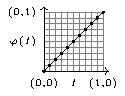
\includegraphics[width=\textwidth]{figures/dyn-prog-full-disc-id/fig.pdf}
        \caption{}
        \label{fig:dyn-prog-full-disc-id}
    \end{subfigure}
    \hfill
    \begin{subfigure}[b]{0.45\textwidth}
        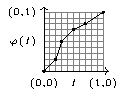
\includegraphics[width=\textwidth]{figures/dyn-prog-full-disc/fig.pdf}
        \caption{}
        \label{fig:dyn-prog-full-disc}
    \end{subfigure}
    \caption[Reparameterization with Full Discretization]{Reparameterization using full discretization. (a) the identity transformation (no change to the original parameterization), and (b) a reparameterized path.}
    \label{fig:dyn-prog}
\end{figure}

The condition \(k < i\) and \(l < j\) ensures the transformation proceeds positively, avoiding loops and maintaining the orientation of \(q_2\).